\section{质点运动学习题解答}
\subsection{直角坐标分量求轨道、速度、加速度}
已知质点的运动方程
\[
x=\sqrt{3}\cos \frac{\pi}{4}t,\quad y=\sin \frac{\pi}{4}t
\]
式中，$x,y$ 以 $\mathrm{m}$ 计，$t$ 以 $\mathrm{s}$ 计。
\begin{enumerate}
    \item 求质点的轨道方程，并在 $xOy$ 平面上描画出质点的轨道；
    \item 求出质点的速度和加速度表示式；
    \item 求 $t=1\ \mathrm{s}$ 时质点的位置、速度和加速度。
\end{enumerate}
\begin{solution}
\begin{enumerate}
    \item \textbf{轨道方程}
由运动方程变形：
\[
\frac{x}{\sqrt{3}} = \cos\frac{\pi}{4}t,\quad y = \sin\frac{\pi}{4}t
\]
利用三角恒等式 $\cos^2\theta+\sin^2\theta=1$：
\[
\boxed{\frac{x^2}{3} + y^2 = 1}
\]
轨道为长半轴 $a=\sqrt{3}$（$x$ 轴）、短半轴 $b=1$（$y$ 轴）的椭圆。
    \item \textbf{速度与加速度表达式}
位置矢量：
\[
\vect{r} = \sqrt{3}\cos\frac{\pi}{4}t\,\vect{i} + \sin\frac{\pi}{4}t\,\vect{j}
\]
速度 $\vect{v}=\dfrac{d\vect{r}}{dt}$：
\[
\begin{aligned}
v_x &= \frac{dx}{dt} = -\frac{\sqrt{3}\pi}{4}\sin\frac{\pi}{4}t,\\
v_y &= \frac{dy}{dt} = \frac{\pi}{4}\cos\frac{\pi}{4}t,\\
\vect{v} &= -\frac{\sqrt{3}\pi}{4}\sin\frac{\pi}{4}t\,\vect{i} + \frac{\pi}{4}\cos\frac{\pi}{4}t\,\vect{j}.
\end{aligned}
\]
加速度 $\vect{a}=\dfrac{d\vect{v}}{dt}$：
\[
\begin{aligned}
a_x &= -\frac{\sqrt{3}\pi^2}{16}\cos\frac{\pi}{4}t = -\frac{\pi^2}{16}x,\\
a_y &= -\frac{\pi^2}{16}\sin\frac{\pi}{4}t = -\frac{\pi^2}{16}y,\\
\vect{a} &= -\frac{\pi^2}{16}\left(\sqrt{3}\cos\frac{\pi}{4}t\,\vect{i}+\sin\frac{\pi}{4}t\,\vect{j}\right)
= -\frac{\pi^2}{16}\vect{r}.
\end{aligned}
\]
    \item \textbf{$t=1\ \mathrm{s}$ 瞬时量}
$\dfrac{\pi}{4}t\big|_{t=1}=\dfrac{\pi}{4}$
\[
\begin{aligned}
&\vect{r}\big|_{t=1} = \sqrt{3}\cos\frac{\pi}{4}\,\vect{i}+\sin\frac{\pi}{4}\,\vect{j}
= \frac{\sqrt{6}}{2}\vect{i} + \frac{\sqrt{2}}{2}\vect{j}\ \mathrm{(m)},\\
&\vect{v}\big|_{t=1} = -\frac{\sqrt{6}\pi}{8}\vect{i}+\frac{\sqrt{2}\pi}{8}\vect{j}\ \mathrm{(m/s)},\\
&\vect{a}\big|_{t=1} = -\frac{\sqrt{6}\pi^2}{32}\vect{i}-\frac{\sqrt{2}\pi^2}{32}\vect{j}\ \mathrm{(m/s^2)}.
\end{aligned}
\]
\end{enumerate}
\end{solution}
\subsection{\texorpdfstring{变加速度 $a=-kv^2$ 积分求速度}{变加速度a=-kv^2积分求速度}}
一艘正在以 $v_0$ 速率沿直线行驶的电艇，在发动机关闭后，其加速度方向与速度方向相反，大小与速度平方成正比，即 $a=-kv^2$，式中 $k$ 为常量。试求电艇在关闭发动机后又行驶 $x$ 距离时的速度。
\begin{solution}
加速度作变量代换 $a=\dfrac{dv}{dt}=\dfrac{dv}{dx}\cdot\dfrac{dx}{dt}=v\dfrac{dv}{dx}$，代入：
\[
v\frac{dv}{dx} = -kv^2
\]
分离变量（$v\neq0$）：
\[
\frac{dv}{v} = -k\,dx
\]
定积分上下限：初始 $x=0,\,v=v_0$；末态 $x=x,\,v=v$
\[
\int_{v_0}^{v} \frac{dv}{v} = -k\int_{0}^{x}dx
\]
\[
\ln v - \ln v_0 = -kx \implies \ln\frac{v}{v_0}=-kx
\]
\[
\boxed{v = v_0 e^{-kx}}
\]
\end{solution}
\subsection{拉船靠岸的速度、加速度（牵连运动）}
\begin{center}
% 加载波浪线绘图库
\begin{tikzpicture}[scale=1.2, decoration={snake, amplitude=2pt, segment length=6pt}]
% 岸壁
\draw (0,0) -- (0,3);
\draw (-1,3) -- (0,3);
\fill (0,3) circle (2pt) node[above right]{收绳点};
% 高度h标注
\draw[<->] (-0.3,0) -- (-0.3,3) node[midway,left]{$h$};
% 水面波浪线（使用decorate）
\draw[decorate] (0,0) -- (4,0);
% 船位置
\fill (4,0) circle (2pt);
% 绳子
\draw (0,3) -- (4,0);
% 水平距离s
\draw[<->] (0,-0.3) -- (4,-0.3) node[midway,below]{$s$};
% 收绳速度v0
\draw[<-] (-0.8,3) -- (-0.2,3) node[above]{$v_0$};
\end{tikzpicture}
\end{center}
在离水面高度为 $h$ 的岸壁上，有人用绳子拉船靠岸，船位于离岸壁 $s$ 距离处，当以 $v_0$ 的速度收绳时，试问船的速度、加速度的大小各为多少？
\begin{solution}
设绳长为 $l$，几何关系：$l=\sqrt{h^2+s^2}$
收绳速率：$\dfrac{dl}{dt}=-v_0$（绳长缩短，导数为负）
船的位置坐标为 $s$，船速 $v=\dfrac{ds}{dt}$
两边对 $t$ 求导：
\[
\frac{dl}{dt} = \frac{s}{\sqrt{h^2+s^2}} \cdot \frac{ds}{dt}
\]
\[
-v_0 = \frac{s}{l}\,v \implies v = -\frac{l}{s}v_0 = -\frac{\sqrt{h^2+s^2}}{s}\,v_0
\]
船速大小（指向岸，速率）：
\[
\boxed{|v| = \frac{\sqrt{h^2+s^2}}{s}\,v_0}
\]
加速度 $a=\dfrac{dv}{dt}$：
\[
v = -v_0 (h^2+s^2)^{\frac12} s^{-1}
\]
\[
\frac{dv}{dt} = -v_0 \cdot \frac{s\cdot \dfrac{s}{\sqrt{h^2+s^2}} - \sqrt{h^2+s^2}}{s^2} \cdot \frac{ds}{dt}
\]
\[
\frac{dv}{dt} = -v_0 \cdot \frac{s^2-(h^2+s^2)}{s^2\sqrt{h^2+s^2}} \cdot v
= -v_0 \cdot \frac{-h^2}{s^2\sqrt{h^2+s^2}} \cdot \left(-\frac{\sqrt{h^2+s^2}}{s}v_0\right)
\]
\[
\boxed{a = -\frac{h^2 v_0^2}{s^3}}
\]
负号表示加速度指向河岸，加速度大小：$\boldsymbol{\dfrac{h^2 v_0^2}{s^3}}$。
\end{solution}
\subsection{鼓轮匀角加速转动，求C点速度加速度}
\begin{center}
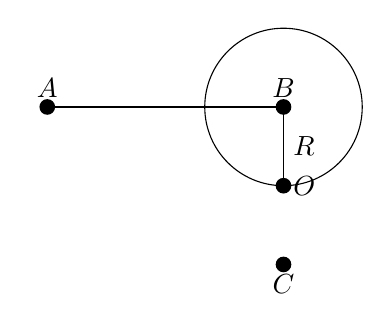
\begin{tikzpicture}[scale=1]
\draw (-3,2) node[circle,fill,inner sep=2pt]{} node[above]{$A$} -- (0,2) node[circle,fill,inner sep=2pt]{} node[above]{$B$};
\draw (0,2) circle (1);
\draw (0,2) -- (0,1) node[circle,fill,inner sep=2pt]{} node[right]{$O$} node[midway,right]{$R$};
\draw (0,0) node[circle,fill,inner sep=2pt]{} node[below]{$C$};
\end{tikzpicture}
\end{center}
一卷扬机的鼓轮自静止开始作匀角加速度转动，水平绞索上的 $A$ 点经 $3\ \mathrm{s}$ 后到达鼓轮边缘上的 $B$ 点处。已知 $AB=0.45\ \mathrm{m}$，鼓轮半径 $R=0.5\ \mathrm{m}$。求 $A$ 点到达最低点 $C$ 时的速度与加速度。
\begin{solution}
\textbf{修正说明：A点随绞索先水平匀加速直线运动，缠绕上鼓轮后做匀角加速圆周运动，切向加速度保持不变。}
1. 水平段 $AB$：初速度为0匀加速直线运动
\[
s_{AB} = \frac12 a_t t_1^2 \implies 0.45 = \frac12 a_t \cdot 3^2
\]
\[
a_t = \frac{2\times 0.45}{9} = 0.1\ \mathrm{m/s^2}
\]
2. 鼓轮匀角加速关系：$a_t = R \beta \implies \beta = \dfrac{a_t}{R} = \dfrac{0.1}{0.5}=0.2\ \mathrm{rad/s^2}$
$A$ 由B转到最低点C，转过圆心角 $\theta=\pi$，匀角加速转动：
\[
\omega_C^2 - \omega_B^2 = 2\beta \pi
\]
先求B点角速度：$\omega_B = \dfrac{v_B}{R},\ v_B = a_t t_1 = 0.1\times3 = 0.3\ \mathrm{m/s}$
\[
\omega_B = \frac{0.3}{0.5}=0.6\ \mathrm{rad/s}
\]
\[
\omega_C^2 = 0.6^2 + 2\times 0.2 \times \pi = 0.36 + 0.4\pi
\]
3. C点线速度：
\[
v_C = R \omega_C = 0.5 \sqrt{0.36+0.4\pi} \approx 0.5 \times 1.351 = \boxed{0.676\ \mathrm{m/s}}
\]
4. 加速度分解：
切向加速度全程不变：$a_t=0.1\ \mathrm{m/s^2}$；
法向（向心）加速度：
\[
a_n = \frac{v_C^2}{R} = \frac{R^2\omega_C^2}{R}=R\omega_C^2 = 0.5(0.36+0.4\pi)\approx 0.456\ \mathrm{m/s^2}
\]
合加速度大小：
\[
a = \sqrt{a_t^2+a_n^2}
= \sqrt{0.1^2 + 0.456^2}
\approx \boxed{0.467\ \mathrm{m/s^2}}
\]
\end{solution}
\subsection{相对运动求风速}
有人以 $v=3\ \mathrm{m\cdot s^{-1}}$ 的速率向东奔跑，他感到风从北方吹来；当奔跑的速率加倍时，则感到风从东北方向吹来，求风的速度。
\begin{solution}
建立坐标系：东为 $x$ 正方向，北为 $y$ 正方向。设风速 $\vect{u}=u_x \vect{i}+u_y\vect{j}$。
人的速度 $\vect{v}_\text{人}$，相对风速 $\vect{u}_\text{相对}=\vect{u}-\vect{v}_\text{人}$。
\begin{enumerate}
    \item $v_\text{人}=3\vect{i}$，相对风正北吹来，相对速度无x分量：
    \[
    u_x - 3 = 0 \implies u_x=3\ \mathrm{m/s}
    \]
    \item 速率加倍 $v_\text{人}=6\vect{i}$，风从东北吹来（相对速度指向西南：$u_x-6 <0,\ u_y<0$，x,y分量相等）：
    \[
    u_x-6 = u_y \implies 3-6=u_y \implies u_y=-3\ \mathrm{m/s}
    \]
\end{enumerate}
风速矢量：
\[
\vect{u}=3\vect{i}-3\vect{j}\ \mathrm{(m/s)}
\]
大小：
\[
u=\sqrt{3^2+(-3)^2}=3\sqrt{2}\ \mathrm{m/s}
\]
方向：\textbf{风源自西北方向（西北风，吹向东南）}。
\end{solution}
\subsection{流速与离岸距离成正比的小船渡河轨迹【重点修复】}
河宽为 $l$，水流速与离岸的距离成正比，中心流速最大为 $v_0$，两岸处流速为零。一小船以恒定的相对速度 $v$ 垂直于水流从一岸驶向另一岸。当它驶至河宽的 $1/4$ 处时，发现燃料不足，立即掉头以相对速度 $0.5v$ 垂直于水流驶回原岸，求此船驶往对岸的轨迹及返回到原岸的地点。
\begin{solution}
设垂直河岸为 $y$ 轴（$0\le y\le l$），沿河水流向为 $x$ 轴。
流速分布：$u(y) = \dfrac{2v_0}{l}y$（线性分布，$y=l/2$ 时 $u=v_0$）。
\subsubsection{第一阶段：去程 \texorpdfstring{$0\to l/4$}{0到l/4}，船垂直对岸 \texorpdfstring{$v_y=v$}{vy=v}}
\[
\frac{dy}{dt}=v,\quad \frac{dx}{dt}=u(y)=\frac{2v_0}{l}y
\]
消去 $dt$：$\displaystyle dx = \frac{2v_0}{lv} y\,dy$
积分：
\[
\int_0^x dx = \int_0^y \frac{2v_0}{lv} y'\,dy' \implies \boldsymbol{x=\frac{v_0}{lv}y^2}
\]
去程轨迹为抛物线。到达 $y=l/4$：
\[
x_1 = \frac{v_0}{lv}\left(\frac{l}{4}\right)^2 = \frac{v_0 l}{16v}
\]
\subsubsection{第二阶段：返程 \texorpdfstring{$y=l/4 \to 0$}{y=l/4到0}，船垂直返回 \texorpdfstring{$v_y=-0.5v$}{vy=-0.5v}}
\[
\frac{dy}{dt}=-\frac{v}{2},\quad \frac{dx}{dt}=\frac{2v_0}{l}y
\]
\[
dt = \frac{dy}{-v/2}=-\frac{2dy}{v}
\]
代入x方向微分：
\[
dx = \frac{2v_0}{l}y \cdot \left(-\frac{2dy}{v}\right) = -\frac{4v_0}{lv} y\,dy
\]
积分上下限：$x:x_1 \to x_\text{总},\ y:l/4 \to 0$
\[
\int_{x_1}^{x_\text{总}} dx = \int_{l/4}^{0} -\frac{4v_0}{lv}\,y\,dy
\]
右侧积分：
\[
\int_{l/4}^{0} -\frac{4v_0}{lv}y\,dy
= -\frac{4v_0}{lv}\cdot\left.\frac{y^2}{2}\right|_{l/4}^{0}
= -\frac{2v_0}{lv}\left(0-\frac{l^2}{16}\right) = \frac{v_0 l}{8v}
\]
\[
x_\text{总} - x_1 = \frac{v_0 l}{8v} \implies x_\text{总} = \frac{v_0 l}{16v}+\frac{2v_0 l}{16v}
\]
\[
\boxed{x_\text{总} = \frac{3v_0 l}{16v}}
\]
即船回到原岸时，在出发点下游 $\boldsymbol{\dfrac{3v_0 l}{16v}}$ 处。
\end{solution}
\subsection{飞机空投救生舱平抛运动}
\begin{center}
\begin{tikzpicture}[scale=1]
% 竖直高度h
\draw (0,5) -- (0,0) node[midway,left]{$h=500\ \mathrm{m}$};
\draw[->] (0,5) -- (2,5) node[above]{$v_0$};
% 平抛抛物线
\draw[thick,domain=0:4] plot (\x,{5 - 0.3125*\x*\x}) node[midway,above]{轨道};
% 视线斜线
\draw[dashed] (0,5) -- (4,0) node[midway,right]{视线};
% 地面
\draw (-1,0) -- (5,0);
\end{tikzpicture}
\end{center}
一架营救飞机以 $198\ \mathrm{km\cdot h^{-1}}$ 的速率在 $500\ \mathrm{m}$ 高处向落水者正上方飞去。
\begin{enumerate}
    \item 释放救生舱时，驾驶员视线与竖直方向夹角多大？
    \item 救生舱落地时速度大小与方向。
\end{enumerate}
\begin{solution}
先单位换算：
\[
v_0 = 198\ \mathrm{km/h} = 55\ \mathrm{m/s},\quad h=500\ \mathrm{m},\ g=9.8\ \mathrm{m/s^2}
\]
\begin{enumerate}
    \item \textbf{下落时间}
竖直自由下落：
\[
h = \frac12 g t^2 \implies t=\sqrt{\frac{2h}{g}}
=\sqrt{\frac{1000}{9.8}}\approx 10.10\ \mathrm{s}
\]
水平射程：
\[
x = v_0 t = 55 \times 10.10 \approx 555.5\ \mathrm{m}
\]
设竖直偏角为 $\theta$：
\[
\tan\theta = \frac{x}{h} = \frac{555.5}{500}\approx 1.111
\]
\[
\boxed{\theta \approx 48.0^\circ}
\]
    \item \textbf{落地速度}
水平分量：$v_x=v_0=55\ \mathrm{m/s}$
竖直分量：
\[
v_y = gt = \sqrt{2gh} = \sqrt{2\times9.8\times500}\approx98.99\ \mathrm{m/s}
\]
合速度大小：
\[
v=\sqrt{v_x^2+v_y^2}
=\sqrt{55^2+98.99^2}\approx \boxed{113.3\ \mathrm{m/s}}
\]
速度与竖直方向夹角 $\alpha$：
\[
\tan\alpha = \frac{v_x}{v_y} \approx \frac{55}{98.99} \implies \alpha\approx 29.1^\circ
\]
\end{enumerate}
\end{solution}
